\section{Point Mass}
The first system model to test was the simple point mass as stated in chapter \ref{ch:Approach}.
While this implementation is a simple version it does already work surprisingly good.
The mean error over the whole flight is normally around 4-5 meter.
It has to be said that this only works while no sensor has a greater offset.
Therefore these values come at the cost that they are not that trustworthy, 
because the system noise on the acceleration has to be set to a greater value to get those good estimation.
An additional factor is also the pitch angle which does hinder this estimation if it changes in a great manner.
This can be seen in figure \ref{fig:PointMassErrorWithOffset} which shows the state estimation error with different offsets.

\begin{figure}[h!]
 \centering
 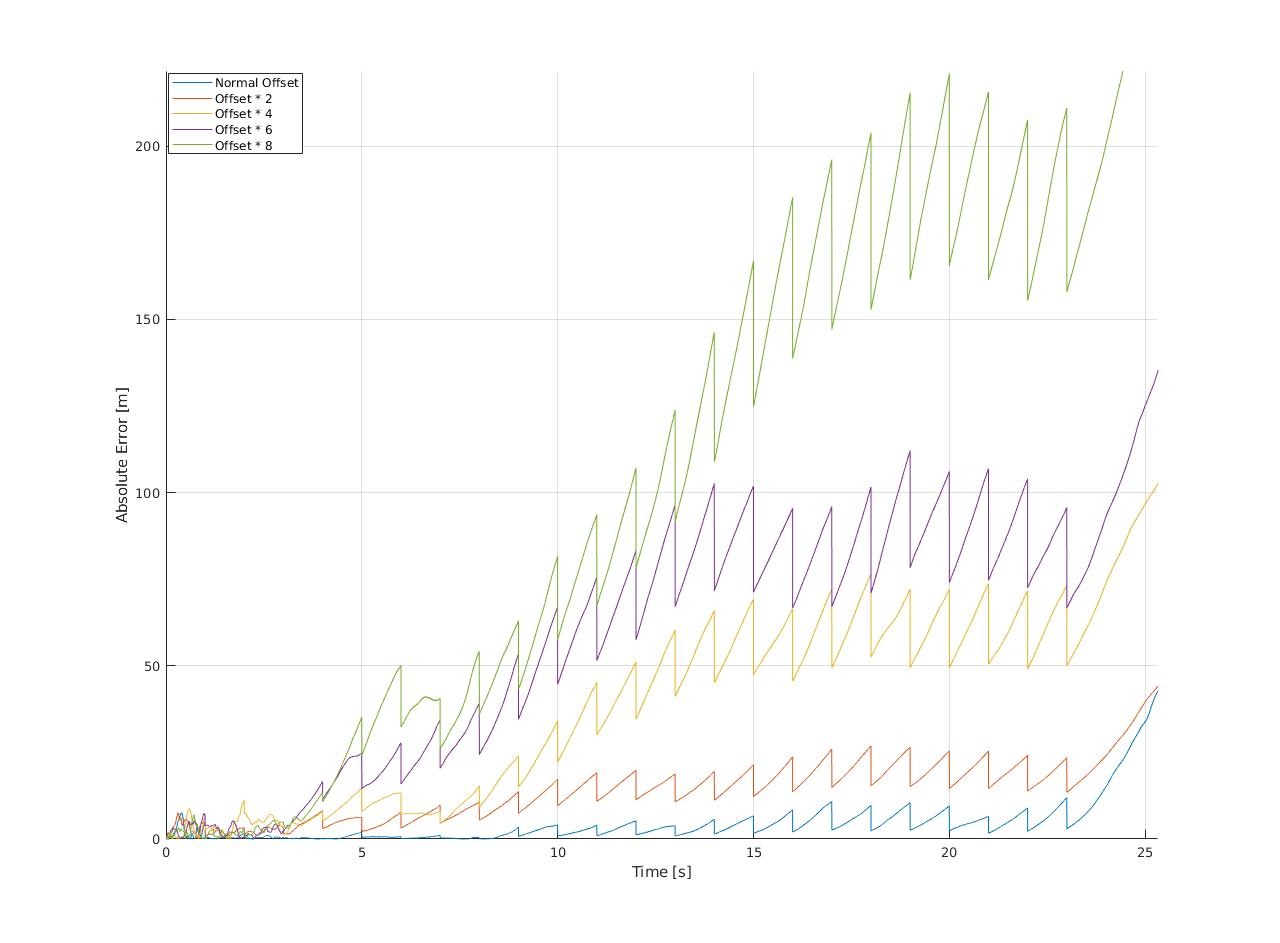
\includegraphics[width=.8\textwidth]{./Pictures/PointMassErrorWithOffset.jpg}
 % PointMassErrorWithOffset.jpg: 0x0 pixel, 300dpi, 0.00x0.00 cm, bb=
 \caption{Error during flight time with different offsets}
 \label{fig:PointMassErrorWithOffset}
\end{figure}


The table %\ref{}
shows the mean and median of the error in the height depending on the offset on the accelerometer.
\begin{center}
\begin{tabular}{ccc}
& Mean & Median\\
Normal & 4.57 & 2.80\\
2Times & 13.97 & 14.66\\
4Times & 39.31 & 46.99\\
6Times & 59.35 & 71.90\\
8Times & 107.21 & 102.15
\end{tabular}
\end{center}

This shows that the error which the estimator makes does rise exponentially.

\subsection{Performance}
%% Add a performance table like max min mean median error under different circumstances. With offsets 
% Discuss pros and cons like not that good estimation but small system load 


\section{Point Mass with Acceleration Offset}
While this system works also sometimes no so good as the first most times it works much better and therefore this should be implemented in the final system.
Like above the figure \ref{fig:PointMassOffsetErrorWithOffset} shows the error during a flight with different sensor offsets.
It can clearly be seen that while the mean error does rise about some value, it always get back to zero and therefore overall this system preforms better as the simple point mass.

\begin{figure}[h!]
 \centering
 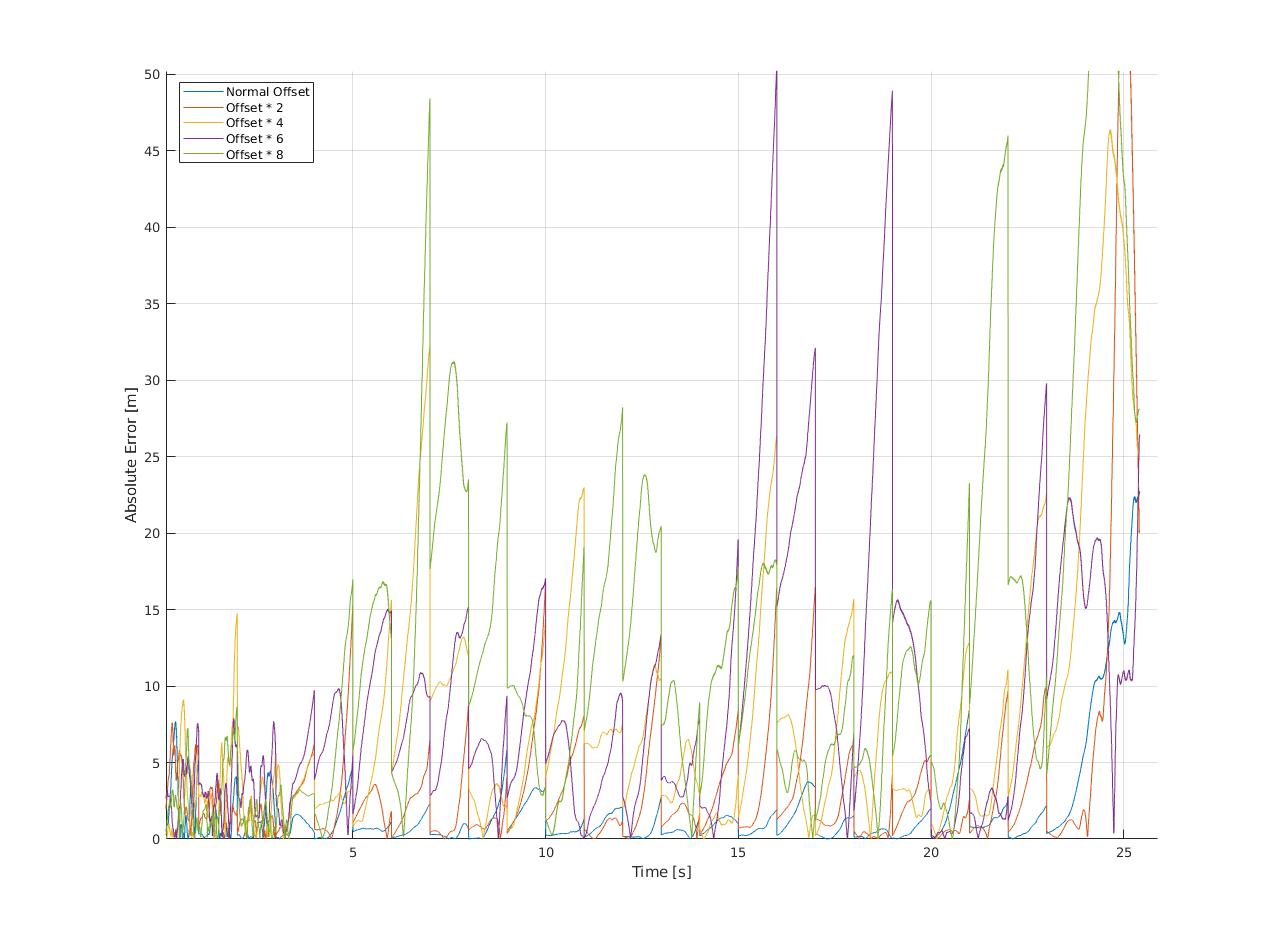
\includegraphics[width=0.8\textwidth]{./Pictures/PointMassOffsetErrorWithOffset.jpg}
 % PointMassOffsetErrorWithOffset.jpg: 0x0 pixel, 300dpi, 0.00x0.00 cm, bb=
  \caption{Error during flight time with different offsets}
 \label{fig:PointMassOffsetErrorWithOffset}
\end{figure}
 
\subsection{Performance}
While it performes much better than the only point mass system it should be much room for above.


\section{Point Mass with Pressure}
The pressure used as state vector has to be shown that it is not that good as firstly tough.
While it does increase the accuracy it does also increase the needed computational effort.
In addition when the temperature gradient is chosen wrong it deeply effects the estimation like seen in figure.
This is a problem due to the fact that the temperature gradient will most certanly not be correct during the whole flight.
The assumption here is that it will be off around 5 percent.
With this can be seen that the system performance is more ore less the same as the normal point mass system.
Therefore the cost ond problems that can occur outweight the gain here.


It is the opposite a system which uses the pressure in the state vector does normally perform.
This mainly due that the noise on the measurements with the interpolation from the linearized 
factor is worse than the interpolation with just the integrated accelerometer measuremnets.
Therefore this will not be used in the best performance system.

%% Maybe try to make this better

\section{Point Mass with Pitch angle}
The pitch angle is difficult to estimate because it has no measured dependencies on its own.
Therefore the kalman filter does just something like a real time low pass filtering.
So the system noise on the pitch angle has to be as good calculated as possible to optimise its estimation.
On the other hand in this implementation the pitch angle does more of less the same thing as the acceleration offset because of it properties.
Due to that, it should be enough to just implement one of them I think

\section{Point Mass with Acceleration as input}
It can be seen in the plot in figure bla, that the estimated height estimated when the acceleration measurements are taken as a input that they reseamble more or less the exact values as from the normal system.
The difference between int the errors between this system model and the normal point mass model is mostly due rounding errors of the simulation then due to really better estimation.
This can be assumed due to the fact that this system model performs some time slightly better and some time slightly worse than the point mass system-
Therefore there is no real gain in the implemenation this way.
In addition with this version the additional adjustment factor which was the system noise onto the acceleration can not be used.
So it does not really make sense to use this in the final version.

Makes no real difference while losing the possibilitey to make system noise because it is used for the measurment noise.

\section{Point Mass with offset and better calculated system noise}
The better calculated system noise first by accesing it in the second was stated in \ref{Implemention}
This by calculating the discrete system noise matrix with the integration as well as
derive the perfect measurements and then low pass filter them to get better system noise vectors.
This had to be used on a system which uses the acceleration offset as well in the state vector to get fully possible gain out of this implemenation.
Figure bla shows that an over hall better estimation can be achieved with this tactic. 
This mostly due the better system noise vector which are much better estimated this way.
Also the additional effort to access this system model only occurs on the preperation,
while it does have no effect on the computational effort during the flight itself.
Non the less this expansion of the state estimation should be used any time if available.


\section{Best Performance System}
Out of the results from the test above the best fitting system can be defined.
While the pitch angle did not have a positive effect on the estimation, the effect of the pressure as a state variable is also to risky to really use it.
Also acceleration as input does not significantly improve the estimation and will therefore not be used.
Therefore the best system consist out of the additional acceleration offset as a state vector as well as better calculated system noise.

It was tested with and without GPS because it is not sure that this would function

\subsection{With GPS}

\subsection{Without GPS}


\section{Sensor Outfall}
\subsection{GPS Outfall}
\subsection{Barometer Outfall}
\subsection{Accelerometer Outfall}
\subsection{Gyrometer Outfall}